\documentclass[a4paper,12pt,oneside]{book}

%-------------------------------Start of the Preable------------------------------------------------
\usepackage[english]{babel}
\usepackage{blindtext}
%packagr for hyperlinks
\usepackage{hyperref}
\hypersetup{
    colorlinks=true,
    linkcolor=blue,
    filecolor=magenta,      
    urlcolor=cyan,
}

\urlstyle{same}
%use of package fancy header
\usepackage{fancyhdr}
\setlength\headheight{26pt}
\fancyhf{}
%\rhead{
\includegraphics[width=1cm]{logo}}
\lhead{\rightmark}
\rhead{
\includegraphics[width=1cm]{logo}}
\fancyfoot[RE, RO]{\thepage}
\fancyfoot[CE, CO]{\href{http://www.e-yantra.org}{www.e-yantra.org}}

\pagestyle{fancy}

%use of package for section title formatting
\usepackage{titlesec}
\titleformat{\chapter}
  {\Large\bfseries} % format
  {}                % label
  {0pt}             % sep
  {\huge}           % before-code
 
%use of package tcolorbox for colorful textbox
\usepackage[most]{tcolorbox}
\tcbset{colback=cyan!5!white,colframe=cyan!75!black,halign title = flush center}

\newtcolorbox{mybox}[1]{colback=cyan!5!white,
colframe=cyan!75!black,fonttitle=\bfseries,
title=\textbf{\Large{#1}}}

%use of package marginnote for notes in margin
\usepackage{marginnote}

%use of packgage watermark for pages
%\usepackage{draftwatermark}
%\SetWatermarkText{
\includegraphics{logo}}
\usepackage[scale=2,opacity=0.1,angle=0]{background}
\backgroundsetup{
contents={
\includegraphics{logo}}
}

%use of newcommand for keywords color
\usepackage{xcolor}
\newcommand{\keyword}[1]{\textcolor{red}{\textbf{#1}}}

%package for inserting pictures
\usepackage{graphicx}

%package for highlighting
\usepackage{color,soul}

%new command for table
\newcommand{\head}[1]{\textnormal{\textbf{#1}}}


%----------------------End of the Preamble---------------------------------------


\begin{document}

%---------------------Title Page------------------------------------------------
\begin{titlepage}
\raggedright
{\Large eYSIP2017\\[1cm]}
{\Huge\scshape Tiva Based Daughter Board For Firebird V.  \\[.1in]}
\vfill
\begin{flushright}
{\large Ayush Gaurav \\}
{\large Nagesh K. \\}
{\large Piyush Manavar \\}
{\large Saurav Shandilya \\}
{\large Duration of Internship: $ 22/05/2017-07/07/2017 $ \\}
\end{flushright}
{\itshape 2017, e-Yantra Publication}
\end{titlepage}
%-------------------------------------------------------------------------------

\chapter[Project Tag]{Tiva Based Daughter Board For Firebird V.}
\section*{Abstract}
%Give the brief introduction and overview of the project
The objective of the project is to design two daughter boards for firebird V
which has the following features:
\begin{itemize}
	\item Compatible With TIVA based platform.
	\item Must support all the necessary features of firebird.
\end{itemize}
The deliverables expected were
\begin{itemize}
	\item 2 working Daughter boards 
		\begin{itemize}
			\item \textbf{Plug and Play Board} with TIVA launchpad
			\item \textbf{uC based Board} with TM4C123GH6PM Microcontroller.
		\end{itemize}
	\item Hardware and software manual for anyone using it in future.
	\item All the demo codes for assistance.
\end{itemize}
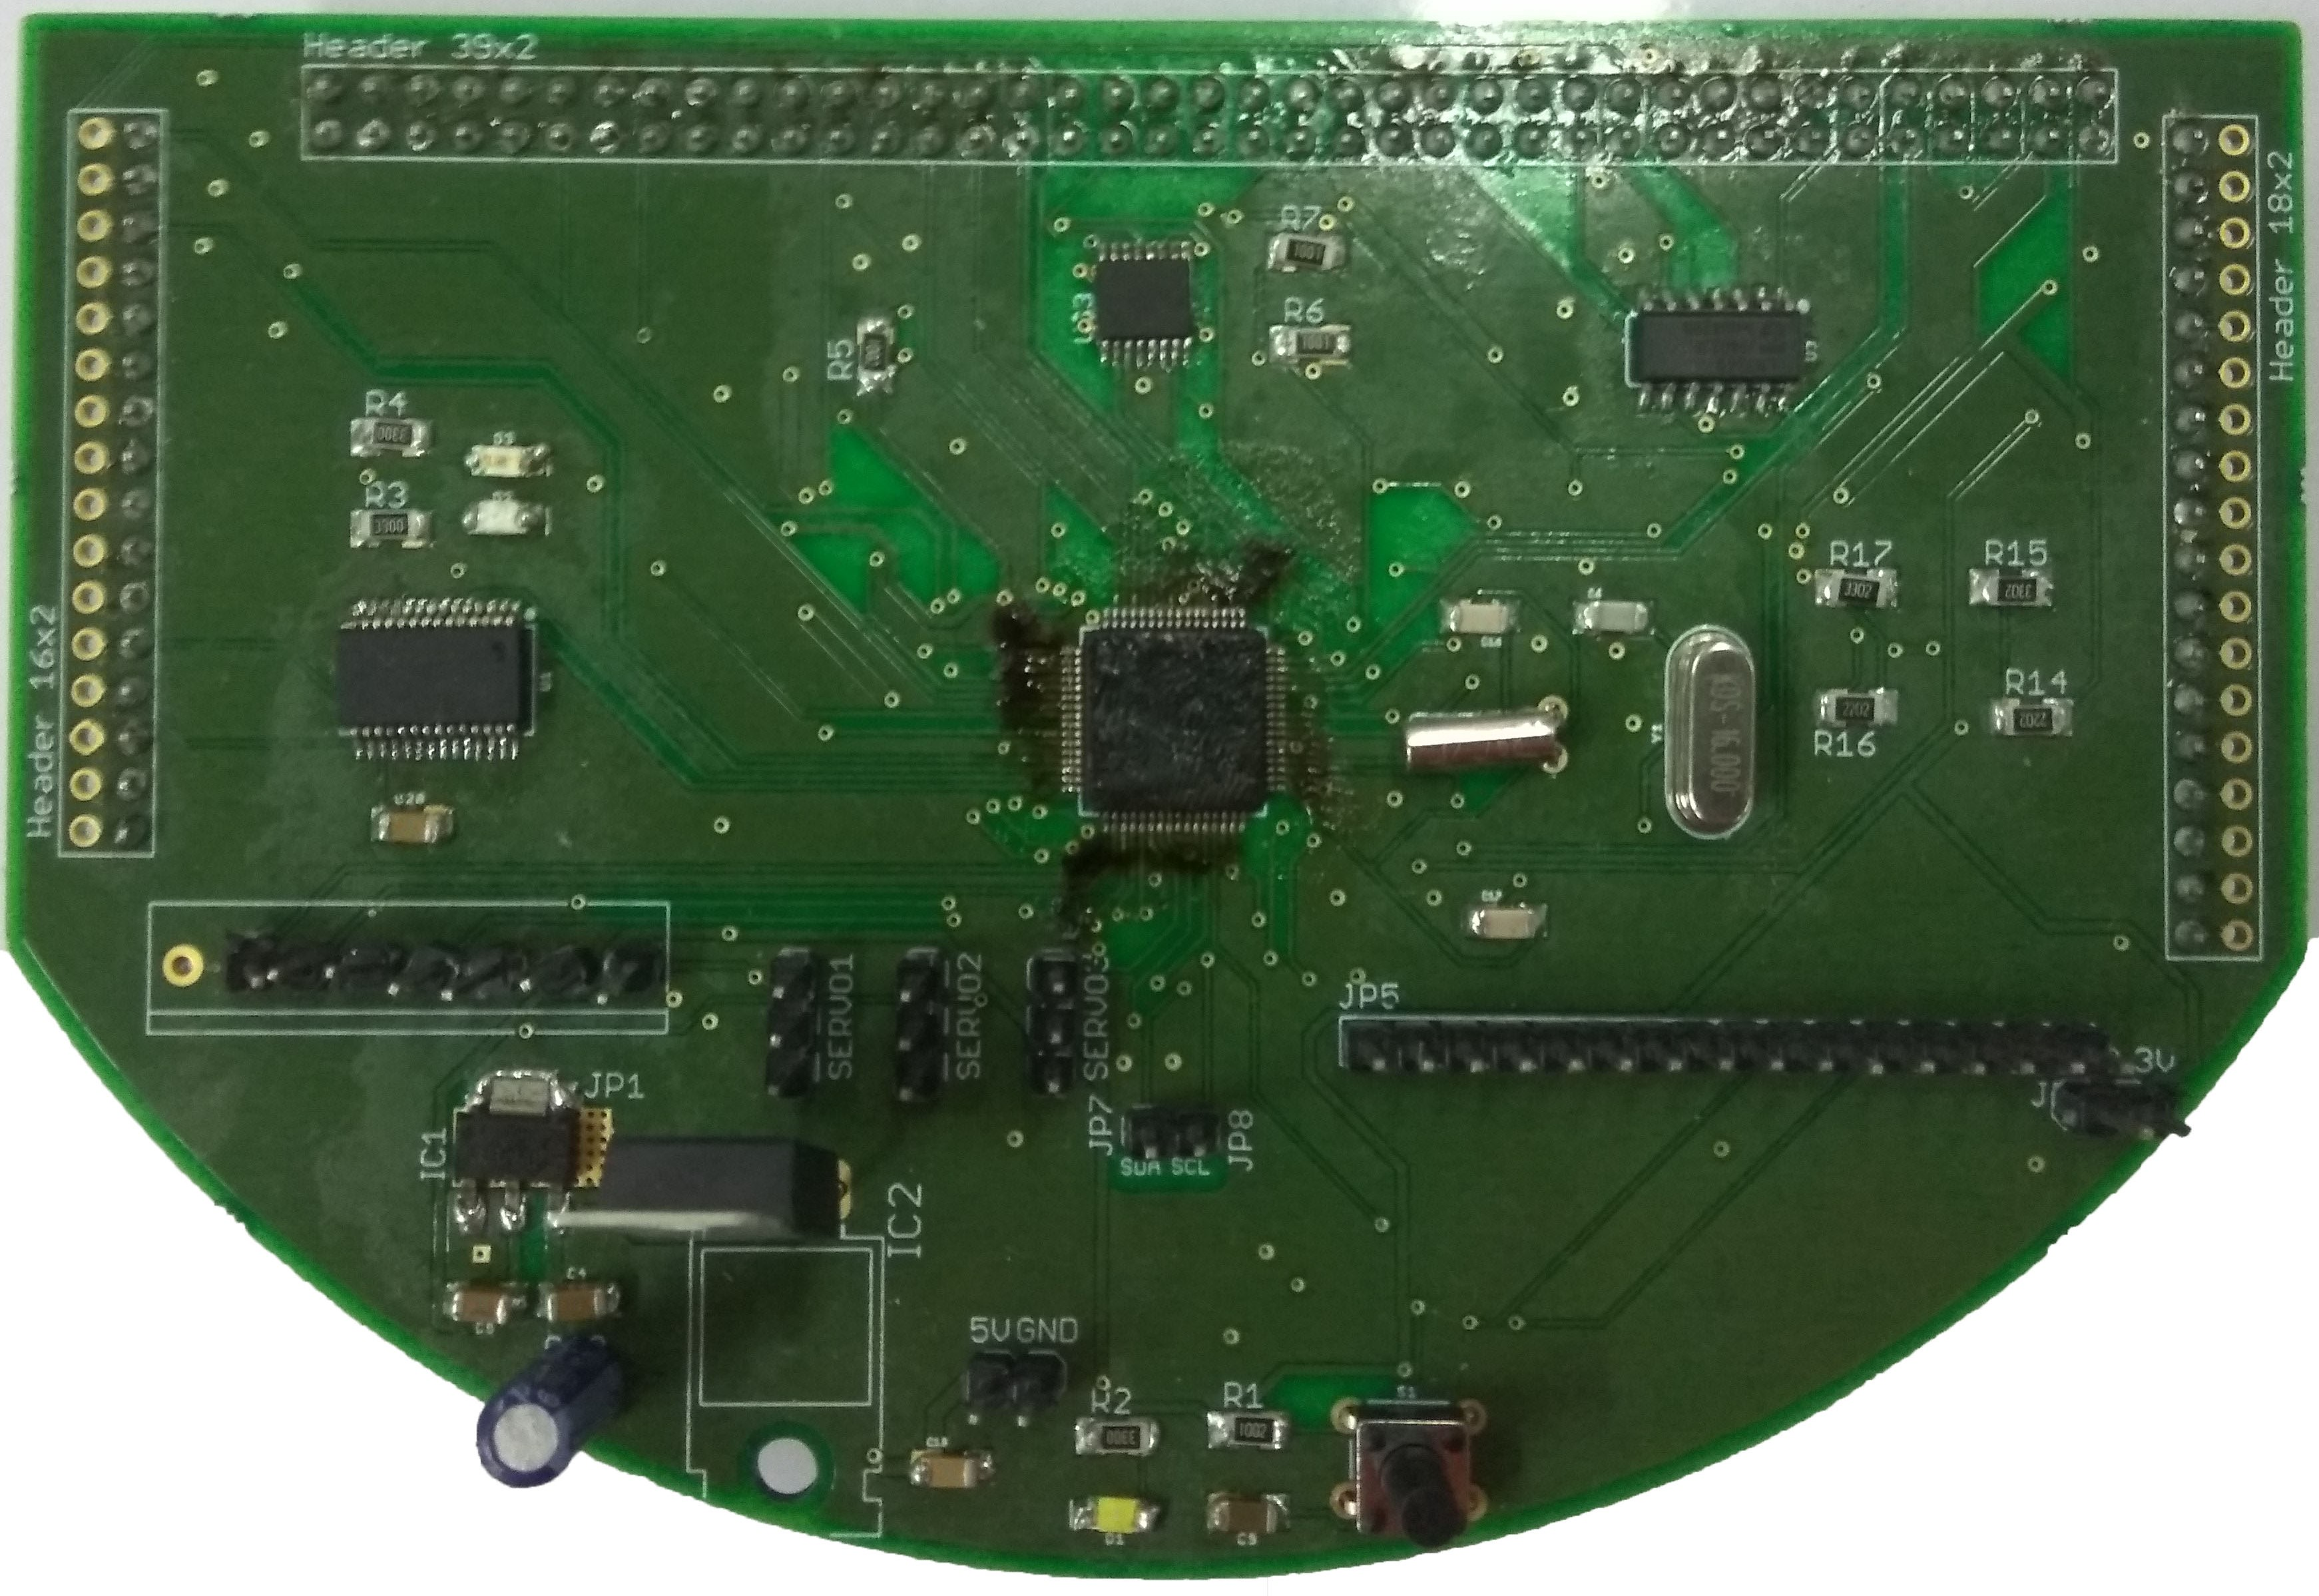
\includegraphics[width=6cm, height=4cm]{Images/uC}
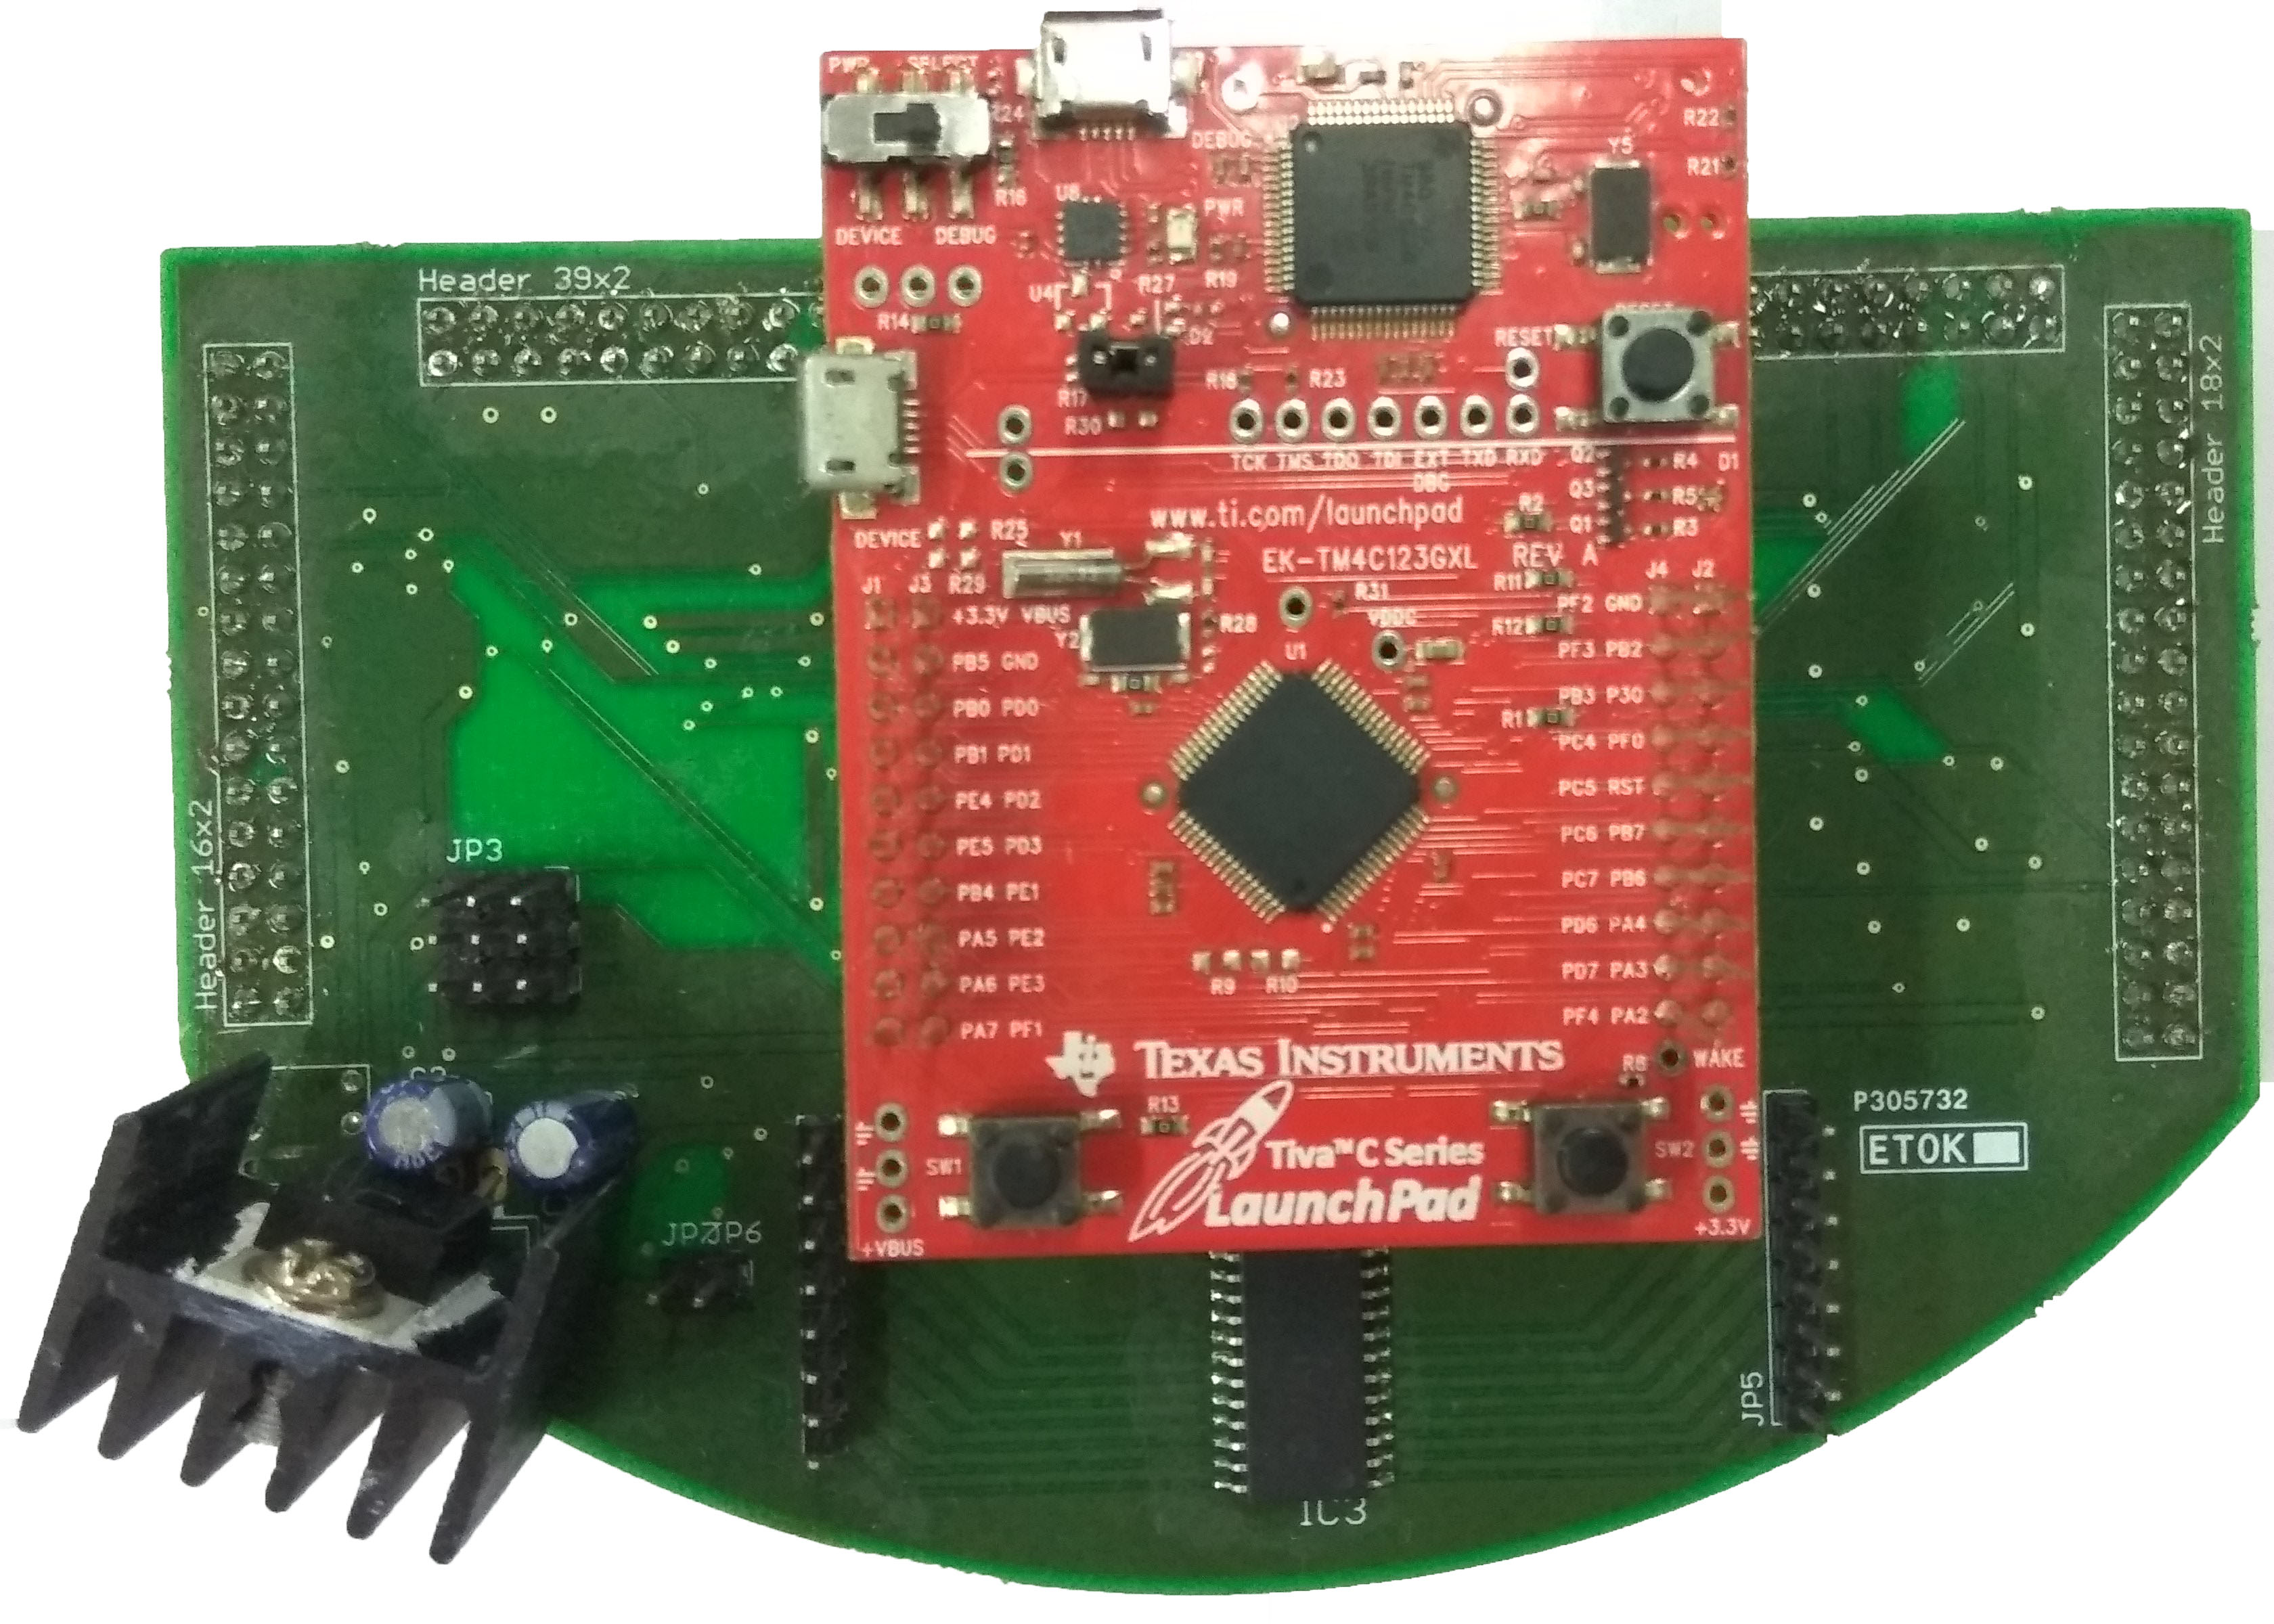
\includegraphics[width=7cm, height=5cm]{Images/PP}\\
Figure1: uC based board
\hspace{2cm}
Figure2: Plug and Play board
\subsection*{Completion status}

%Give details for work/project completed successfully. If work is not
%complete, mention the details till which task is done.
The project was divided in many small tasks which were to be completed in given time. Though we refrain from mentioning that long list but still will give some important one.
\begin{itemize}
	\item Learning Tiva Platform.
	\item Finding solution for limitations offered by Tiva, like limited GPIO pins and limited ADC channels.
	\item Utilizing the functionality provided to the maximum.
	\item Creating schematic and layout for the daughter boards.
	\item Testing the boards and writing all the test codes.
	\item Making hardware and software manuals.
\end{itemize}
\section{Hardware parts}
\begin{itemize}
  \item List of hardware used :
  \begin{itemize}
  	\item Tiva launchpad. 
  	\item TM4C123GH6PM Microcontroller.
  	\item MCP23017 port expander.
  	\item ADC128D818 external ADC.
  	\item Voltage regulator(lm1117,7805).
  	\item FT232
  \end{itemize} 
  \item Detail of each hardware:
  \begin{enumerate}
  	\item Tiva Launchpad: It is a micro-controller  board by Texas Instruments that has on board programmer with real time debugging feature. The micro-controller is very efficient with system clock up to 80MHz and CAN protocol. It has 40 GPIO pins with interrupt on each pin. In addition, it has Two general-purpose user switches, a reset switch, power LED, and user-programmable RGB LED. The tutorial and more information can be read from \href{./datasheet/TIVALaunchpad.pdf}{Datasheet}.
  	\begin{center}
  		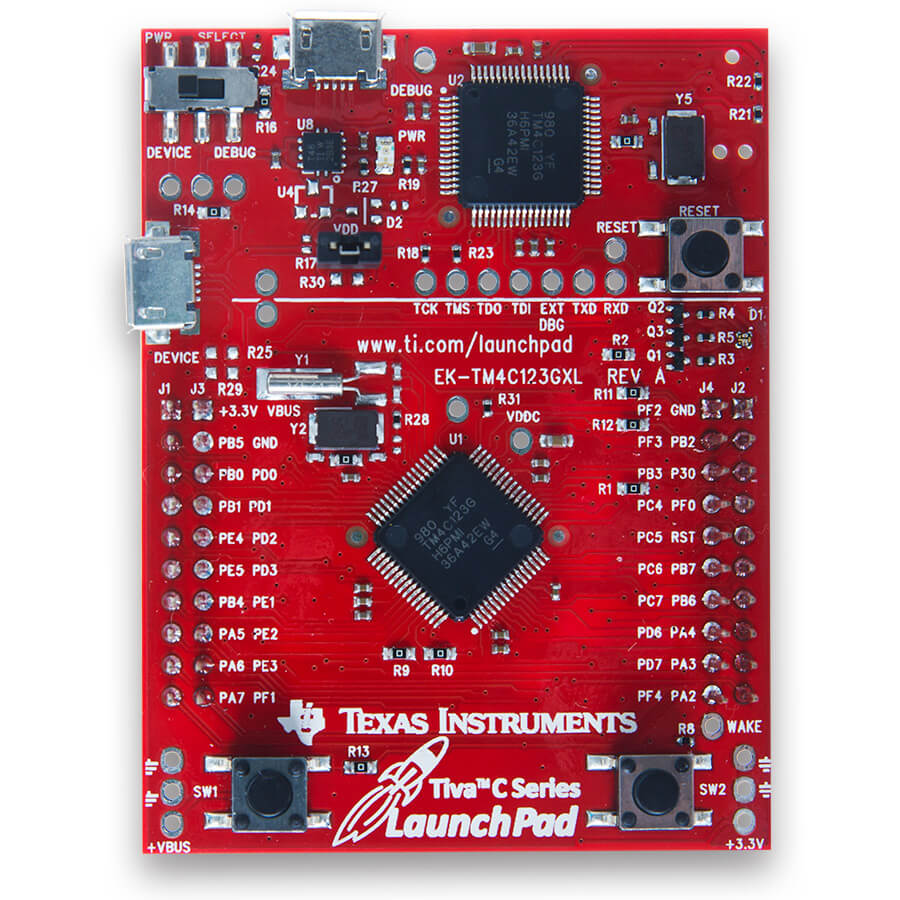
\includegraphics[width=8cm, height=8cm]{Images/launchpad}\\
  		Figure3: TIVA Launchpad\\
  		Picture courtesy: Texas Instruments Manual
  	\end{center}
   			
	\item TM4C123GH6PM is a ARM cortex M4 based micro-controller that is used as a controller of the Tiva Launchpad. It has the following features
		\begin{itemize} 
			\item Upto 80MHz Clock 
			\item 256KB Flash
			\item 32KB RAM
			\item 2-KB EEPROM
			\item On-chip ROM with drivers and boot loaders
			\item 12 channel 12-bit ADCs 
			\item 16 Motion PWM channels
			\item 24 Timer/Counters
			\item 4 SPI/SSI, 2 CAN, 4 I2C, 8 UART
			\item USB Host/Device/OTG
			\item Low-power hibernation mode
			\item 43 GPIO pins
		\end{itemize}	
	 You can read \href{./datasheet/tm4c123gh6pm.pdf}{Datasheet} for more details.
	 \begin{center}
	 	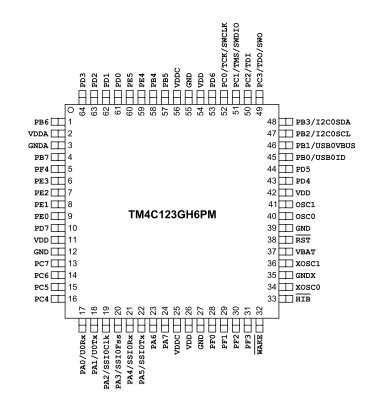
\includegraphics[width=6cm, height=6cm]{Images/TM4C123G}\\
	 	Figure4: TM4C123GH6\\
	 	Picture courtesy: Texas Instruments Manual
	 \end{center}
	
	\item Voltage Regulators:The voltage source available on the Firebird is 9.6V. But the TIVA platform works on 3.3V and the servos can operate up to 6V. So there must be 3 different voltage levels on the board.\\
	The uC based board has 2 voltage regulators. LM117 is used to convert 9.6V to 3.3V and power the microcontroller. 7805 is used for powering the servo motors.\\
	The Plug and Play board has an inbuilt voltage regulator, so it is directly connected to 5V, 300mA source. 7805 is used to convert 9.6V to 5V and power the servo motors.\\
	Datasheets for\href{./datasheet/lm1117.pdf}{3.3 volts regulator LM1117}, and \href{./datasheet/LM7805.pdf}{ 5 volts regulator 7805} 5 volts regulator can be accessed from the links.
	
	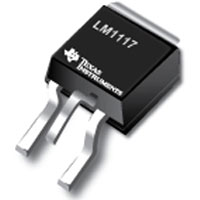
\includegraphics[width=4cm, height=4cm]{Images/LM117}   
	\hspace{2cm}
	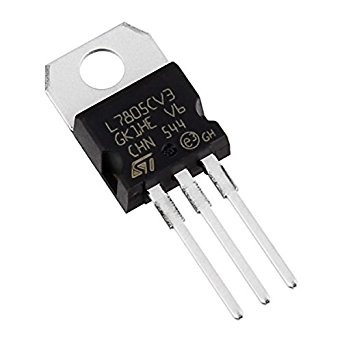
\includegraphics[width=4cm, height=4cm]{Images/7805}\\
	
	Figure5: TM4C123GH6
	\hspace{1.75cm}
	Figure6: TM4C123GH6\\
	Picture courtesy: element14
	\hspace{1cm}
	Picture courtesy: element14
	
	\item Level Converters TIVA platform operates at 3.3V and the Firebird operates at 5V. Directly connecting these pins to the TIVA may be fatal. So for proper level maintenance, a level converter is used. A bidirectional MOS-FET based level converter is used in this case. The level converter is necessary for input pins and may or may not be used in output pins. In the Daughter boards, Level converter is used for interfacing the position encoders of the motors.
	\href{./datasheet/BSS138.pdf}{ Datasheet} of MOSFET is also provided.\\
	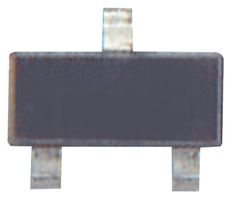
\includegraphics[width=5cm, height=5cm]{Images/BSS138}
	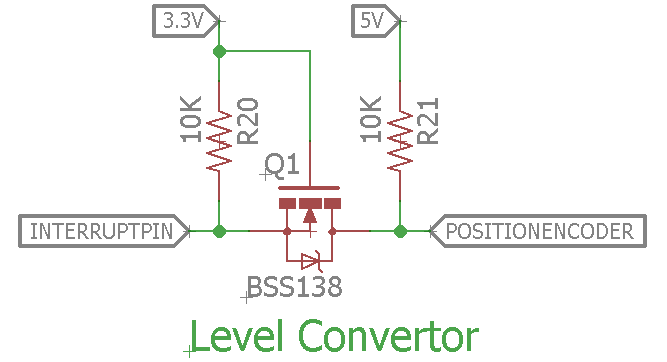
\includegraphics[width=5cm, height=5cm]{Images/Level_Converter}	
	
	Figure7: BSS138
	\hspace{3cm}
	Figure8: Schematic \\ 
	\hspace{6cm}
	Picture Courtesy: element14
	
	\item Port Expander(MCP23017):TM4C123GH6PM has 64 pins out which 43 are GPIO pins. This limits our application to read input and respond correspondingly. To increase the number of GPIO and there interrupts we have
	used I2C compatible a port expander MCP23017. It has 2 PORTS A and B, with each port having 8
	Pins.The interrupts on each pin can also be monitored. To read more about it, download the datasheet
	from here.The schematic of the connection is shown below.Keep in mind that I2C SCL and SDA have
	already been pulled up using 10K resistor.\href{./datasheet/MCP23017.pdf}{ Datasheet} of the port expander can be fount here. 
	\begin{center}
		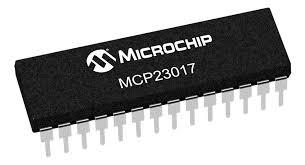
\includegraphics[width=6cm, height=5cm]{Images/MCP23017}\\
		Figure9: MCP23017\\
		Picture Courtesy: Microchip
	\end{center}
	\item FT232 is used for Serial Communication between TM4C123GH6PM and computer. FT232 is used for USB to Serial UART interface. It has an internal oscillator and EEPROM. \\
	This IC is excluded in Plug and Play board as it already has provision for serial communication on board. \\
	\begin{center}
		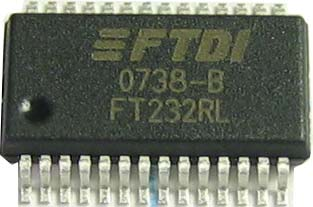
\includegraphics[width=6cm, height=6cm]{Images/FT_232}\\
		Figure10: MCP23017\\
		Picture Courtesy: FTDI
	\end{center} 
	\end{enumerate}  

\end{itemize}

\section{Software used}
\begin{itemize}
  \item \textbf{Autodesk Eagle} can be downloaded from this \href{https://www.autodesk.com/products/eagle/free-download}{link}
  \item \textbf{Installing Autodesk Eagle:}
  		\begin{enumerate}
  			\item Download the installer from the link provided above and run \textit{Autodesk\_EAGLE\_8.0\_English\_Win\_64bit.exe}. 
  			\item Select the Yes button on the next Windows security dialog box.
  			\item Accept the lisence agreement and click on the next button
  				\begin{center}
  					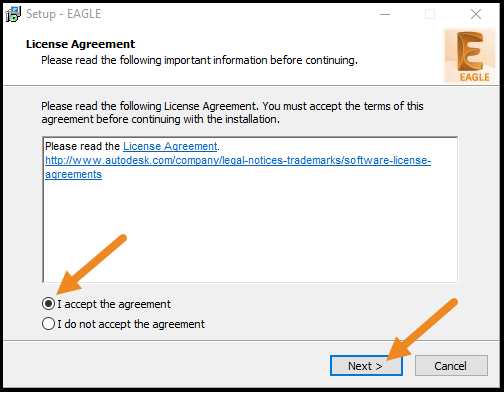
\includegraphics[width=6cm, height=6cm]{Images/E1}\\
  					Figure11
  				\end{center}
  			\item On the final step, click on the \textit{Install} button
				\begin{center}
					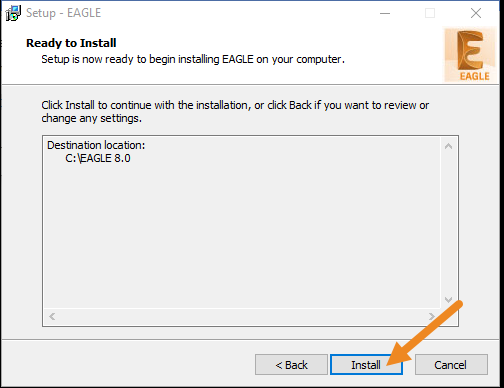
\includegraphics[width=6cm, height=6cm]{Images/E2}\\
					Figure12
				\end{center}  	
			\item With your installation complete go ahead and open Autodesk EAGLE. The first time you run Autodesk EAGLE, you’ll need to sign in to your existing Autodesk account or create a new account. 
				\begin{center}
					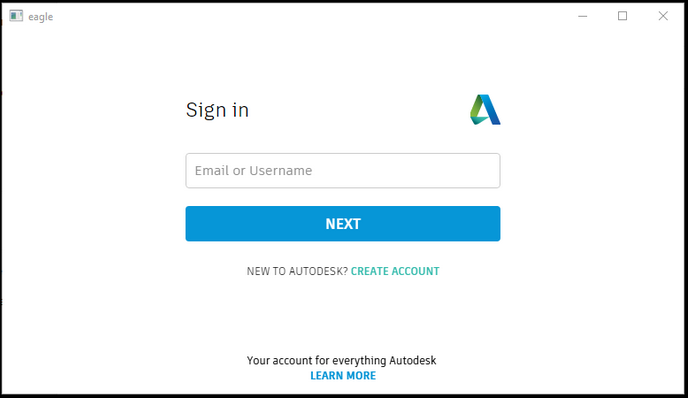
\includegraphics[width=8cm, height=6cm]{Images/E3}\\
					Figure13
				\end{center} 
			
			\textbf{Note:}Autodesk gives free 3 years premium subscription to student lisences.		
  		\end{enumerate}
  
  \item \textbf{Code Composer Studio} version 7.1.0 can be downloaded from this \href{http://processors.wiki.ti.com/index.php/Download_CCS}{link}, 
  \item \textbf{Installing CCS Studio:}


{After the installer has started follow the steps mentioned below:\\
\begin{enumerate}
	\item Accept the Software License Agreement and click Next.\\
	\begin{center}
		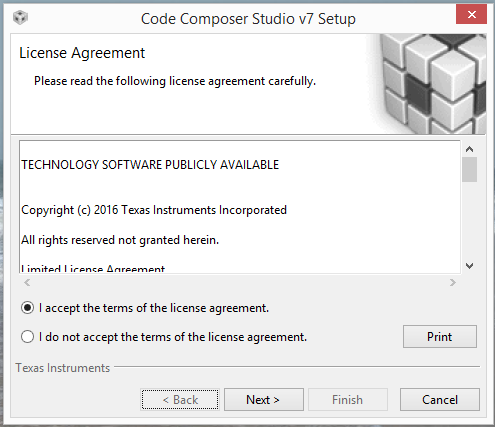
\includegraphics[width=6cm, height=6cm]{Images/CCSInstall1}\\
		Figure14.
	\end{center}
	\item Select the destination folder and click next.\\
	\begin{center}
		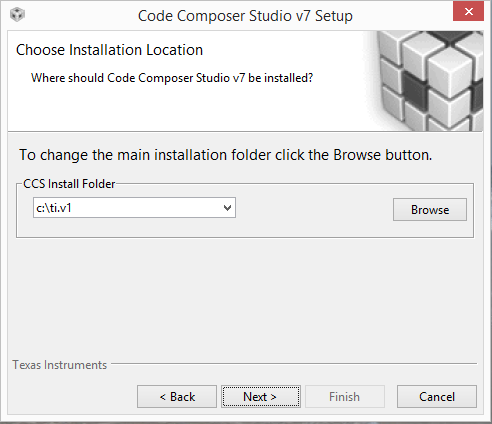
\includegraphics[width=6cm, height=6cm]{Images/CCSInstall2}\\
		Figure15.	
	\end{center}
	\item Select the processors that your CCS installation will support. You
	must select "TM4C12X Arm Cortex M4". You can select other architectures, but the installation time and size will increase.\\
	\begin{center}
		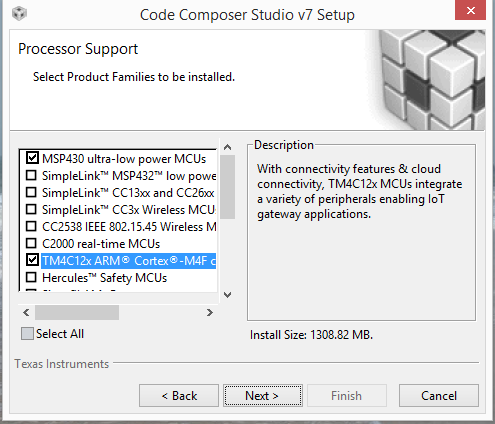
\includegraphics[width=6cm, height=6cm]{Images/CCSInstall3}	\\					Figure16 .
	\end{center}
	\item Select debug probes and click finish \\
	\begin{center}
		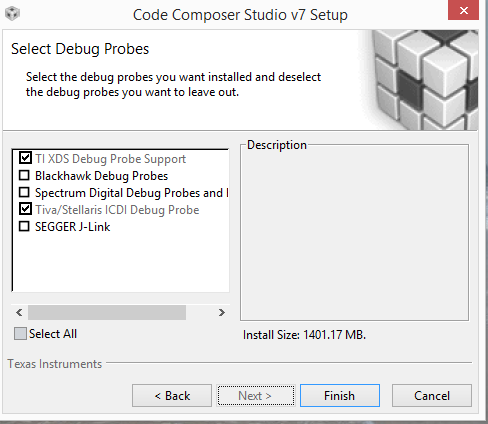
\includegraphics[width=6cm, height=6cm]{Images/CCSInstall4}\\
		Figure17.
	\end{center}
	\item The installer process	should take 15 - 30 minutes, depending on the speed of your connection. The offline
	installation should take 10 to 15 minutes. When the installation is complete, uncheck the
	“Launch Code Composer Studio v7” checkbox and then click Finish.There are several additional tools that require installation during the CCS install process. Click “Yes” or “OK” to proceed when these appear. \\
	\item Install TivaWare for C Series (Complete). Download and install the latest full version of TivaWare from: \href{http://www.ti.com/tool/sw-tm4c}{TivaWare}. The filename is SW-TM4C-x.x.exe . This
	workshop was built using version 1.1. Your version may be a later one. If at all possible,
	please install TivaWare into the default location.
\end{enumerate}}
{\textbf{\\You can find additional information at these websites:}\\
Main page: www.ti.com/launchpad\\
Tiva C Series TM4C123G LaunchPad:\\ http://www.ti.com/tool/ek-tm4c123gxl\\
TM4C123GH6PM folder:\\ http://www.ti.com/product/tm4c123gh6pm\\
BoosterPack webpage: www.ti.com/boosterpack\\
LaunchPad Wiki:\\ www.ti.com/launchpadwiki\\}	\\	
{For understanding the launchpad properly and to learn more about Tiva it is strongly recommended to go through the webpage \href{http://processors.wiki.ti.com/index.php/Getting_Started_with_the_TIVA\%E2\%84\%A2_C_Series_TM4C123G_LaunchPad}{TIva Worshops} and download and read the workbook }

\end{itemize}

\section{Assembly of hardware}

\subsection*{Circuit Diagram}
	\begin{itemize}
		\item \textbf{Plug and Play board} \\
			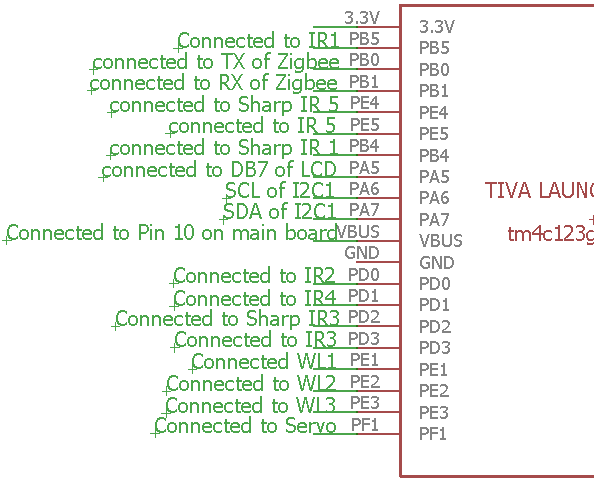
\includegraphics[width=15cm, height=16cm]{Images/PlugandPlay1}
			
			\hspace{6 cm}
			Figure18\\
			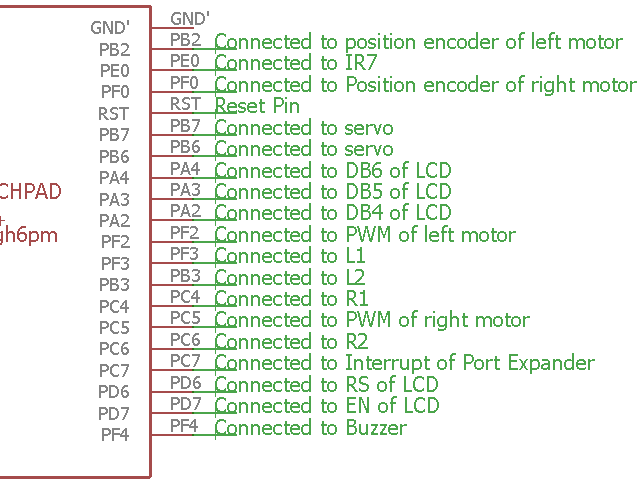
\includegraphics[width=15cm, height=20cm]{Images/PlugandPlay}
			
			\hspace{6 cm}
			Figure19
		\item \textbf{uC based board}\\
			\includegraphics[width=15cm, height=19cm]{Images/uC1}
			
			\hspace{6 cm}
			Figure20\\
			\includegraphics[width=15cm, height=20cm]{Images/uC2}
			
			\hspace{6 cm}
			Figure21
	\end{itemize}
\subsection*{Step 1}
Remove the screws marked in figure using a screw driver. Remove the top cover and carefully unplug the Daughter board.(Use the help of a wedging device if necessary)

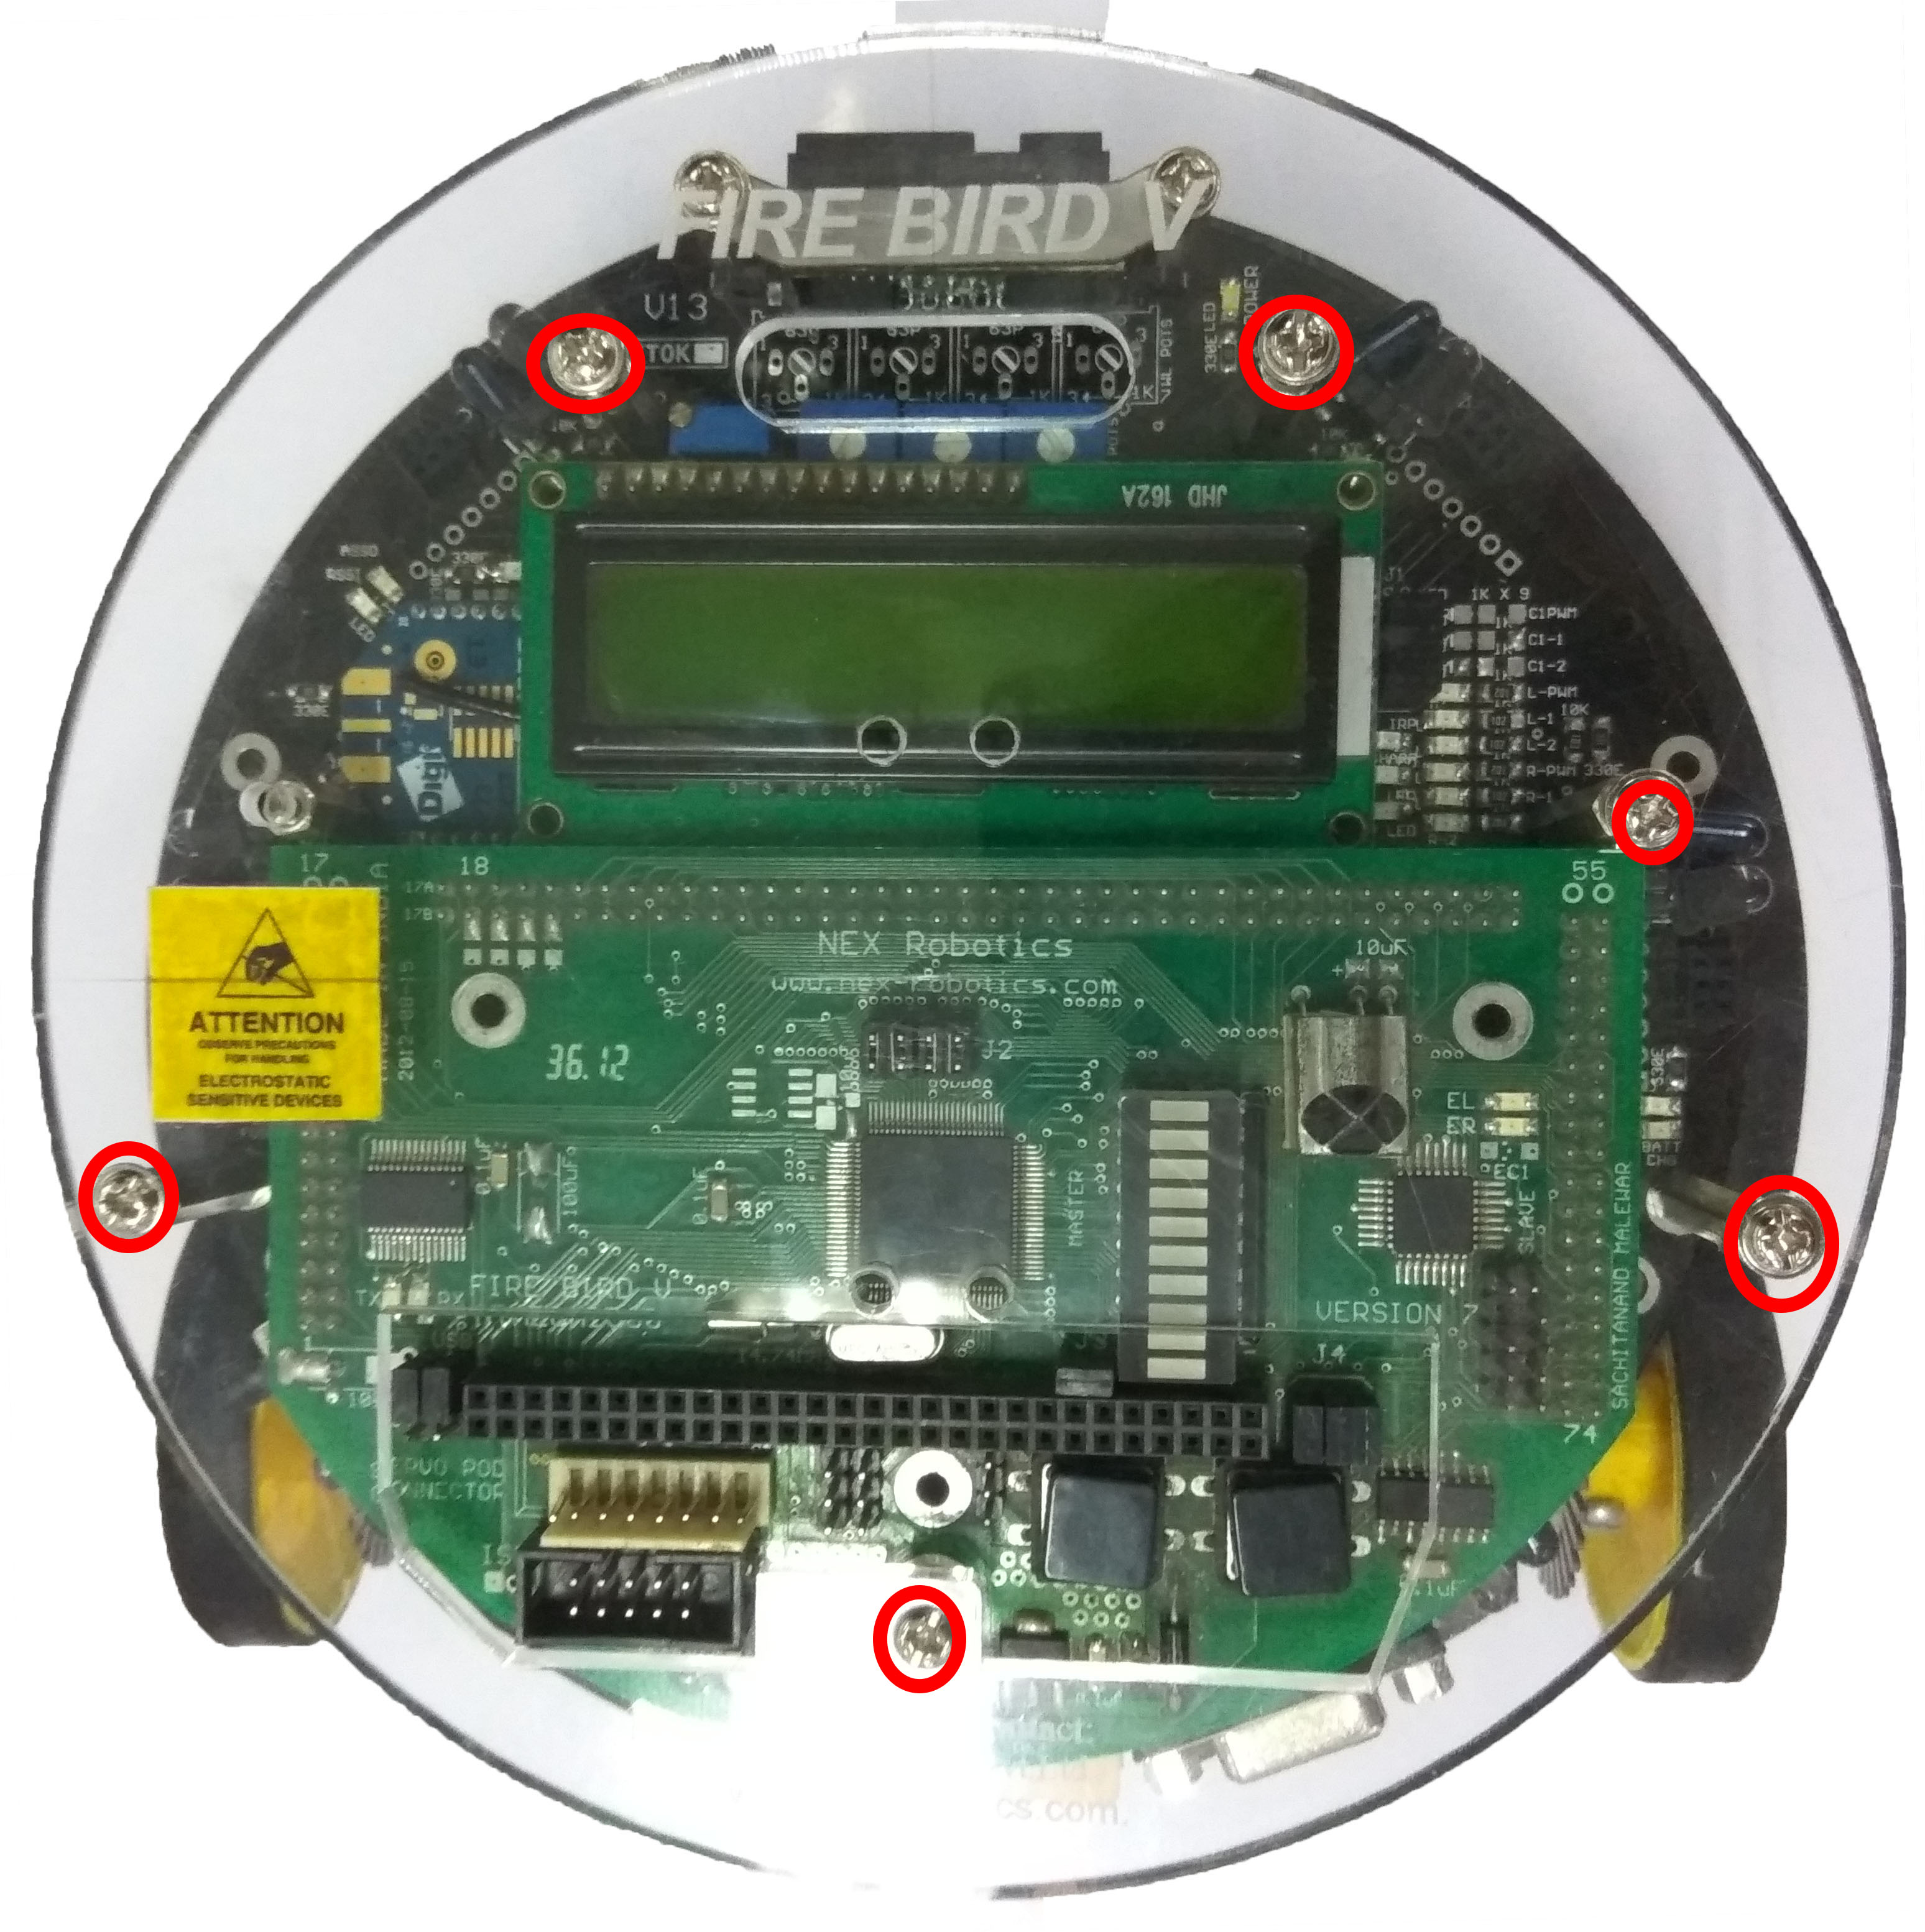
\includegraphics[width=6cm, height=6cm]{Images/1}
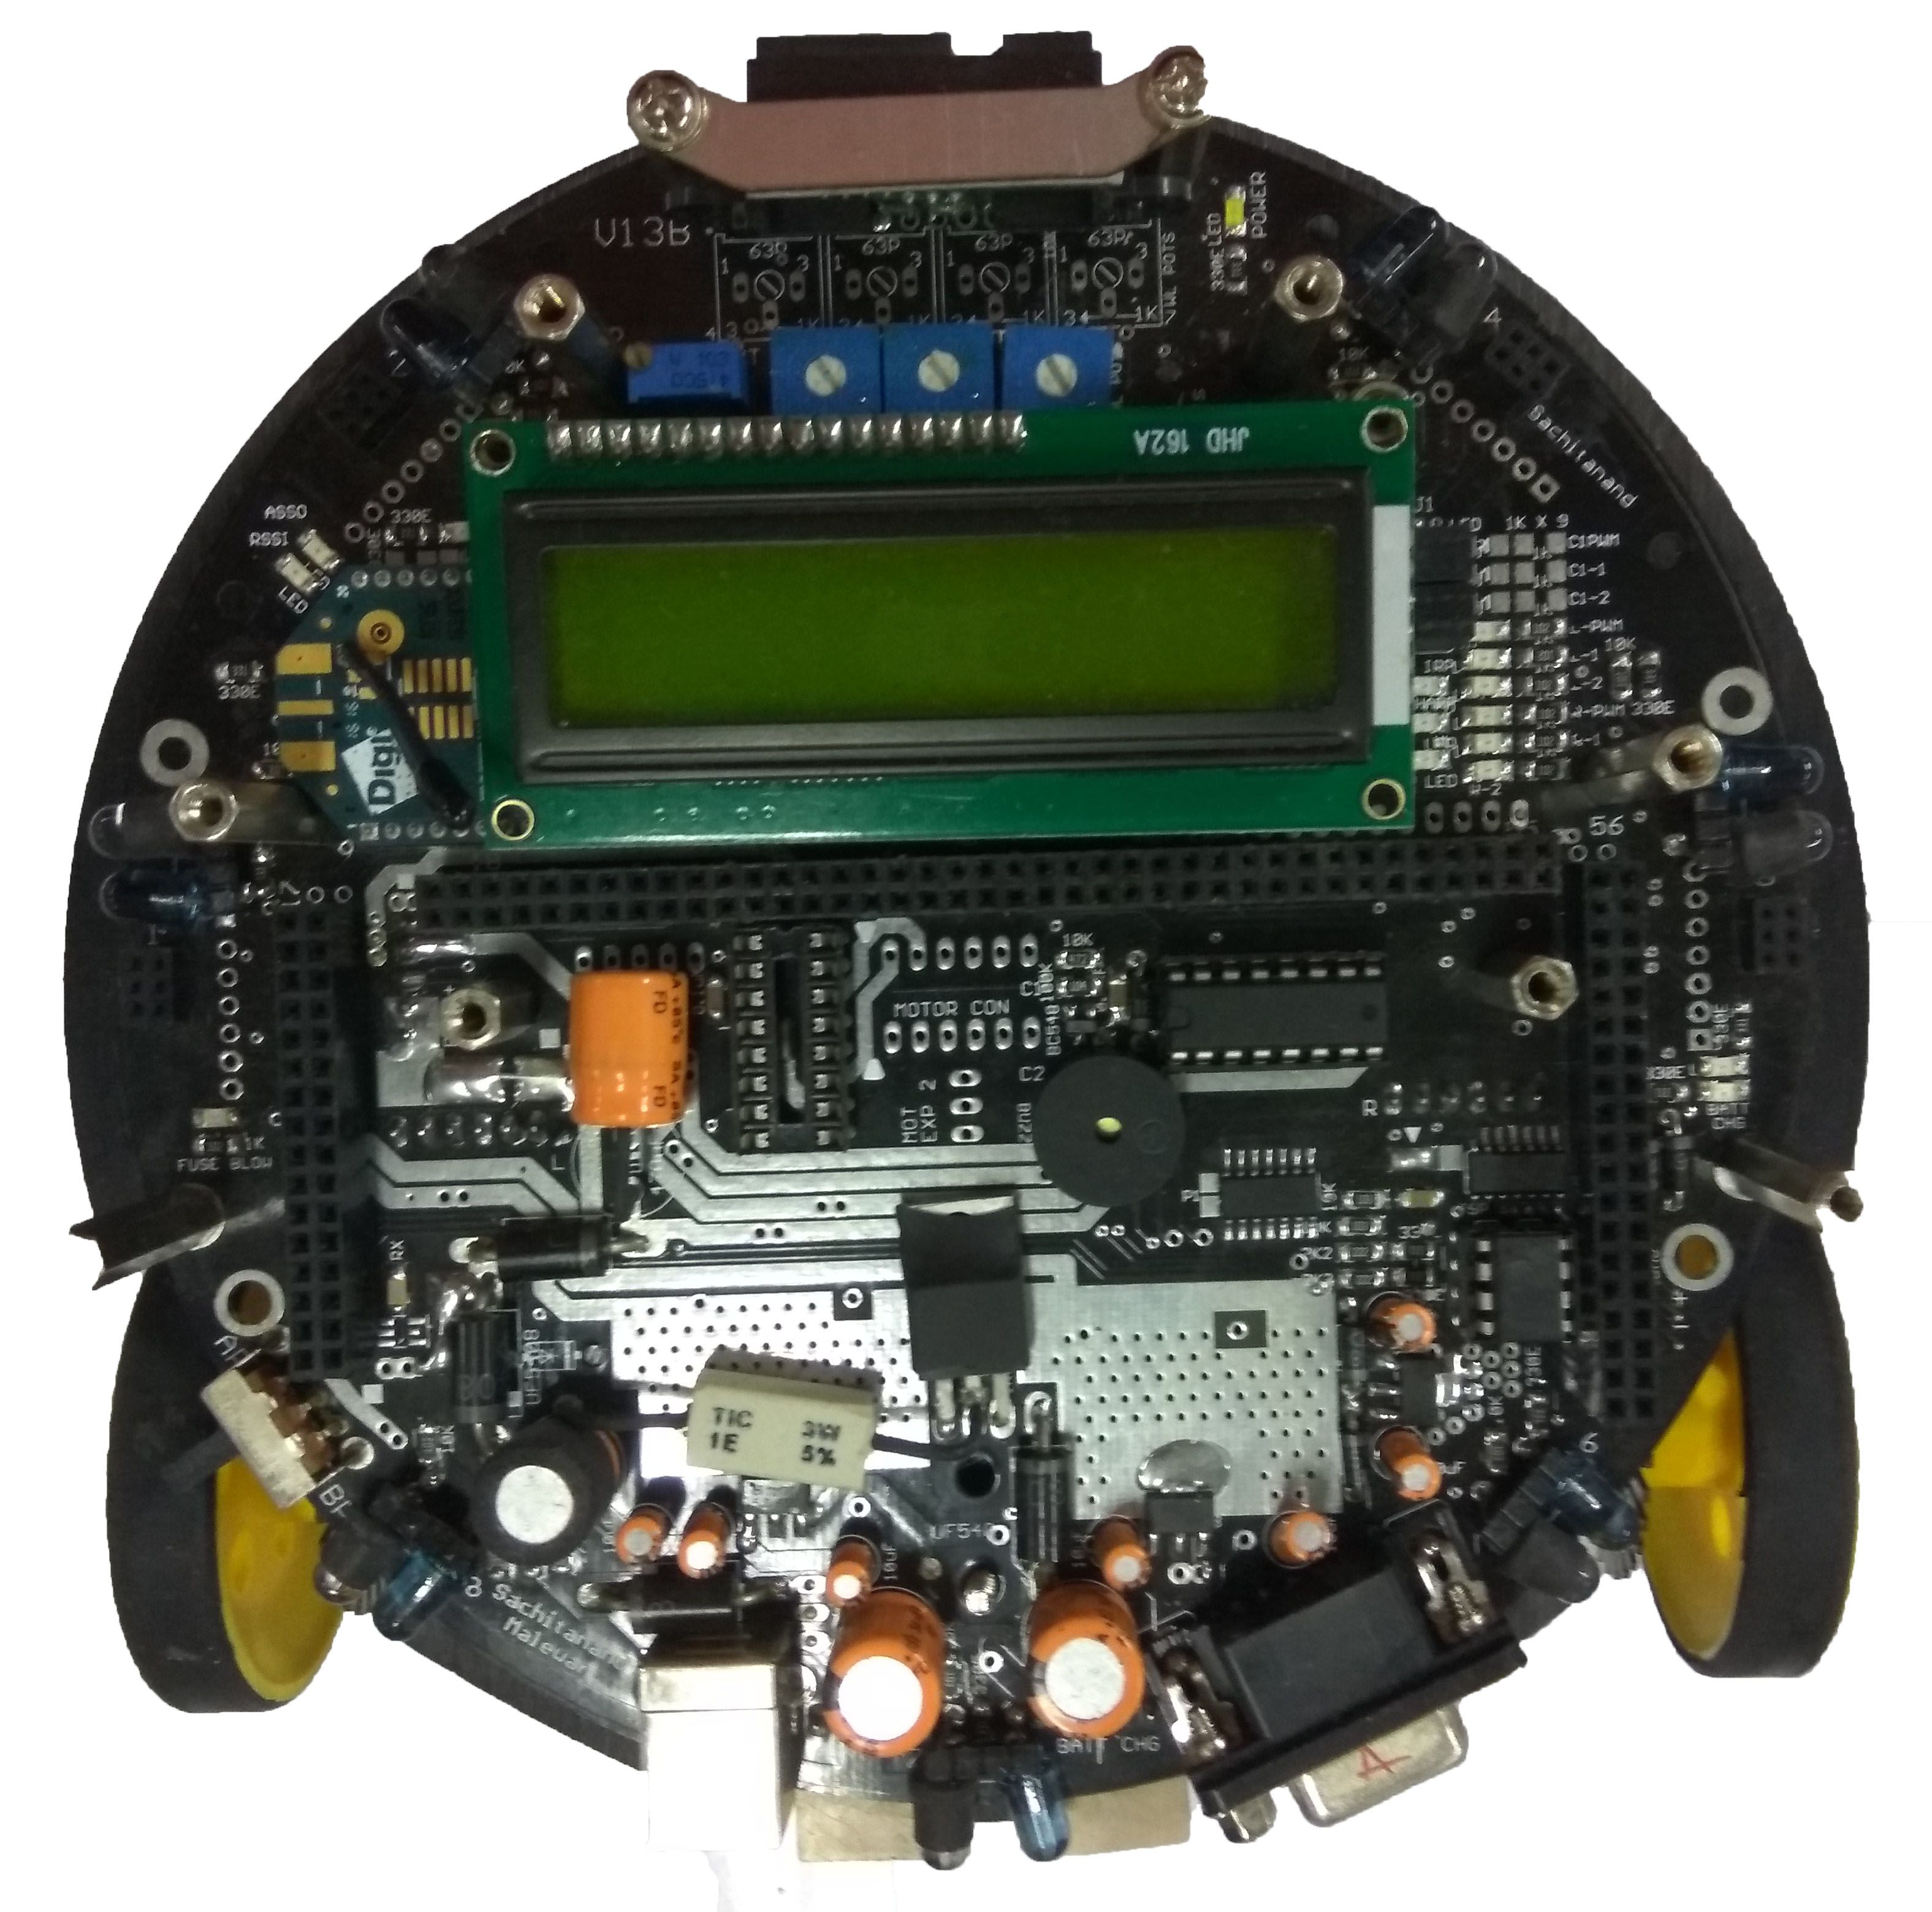
\includegraphics[width=6cm, height=6cm]{Images/2}\\

\hspace{2cm}
Figure22
\hspace{4.5cm}
Figure23

\subsection*{Step 2}
Plug the TIVA based Daughter carefully into slot shown below. Ensure proper allignment of the male burge connector while plugging in the daughter board. The final assembled board looks as shown in figure.\\ 
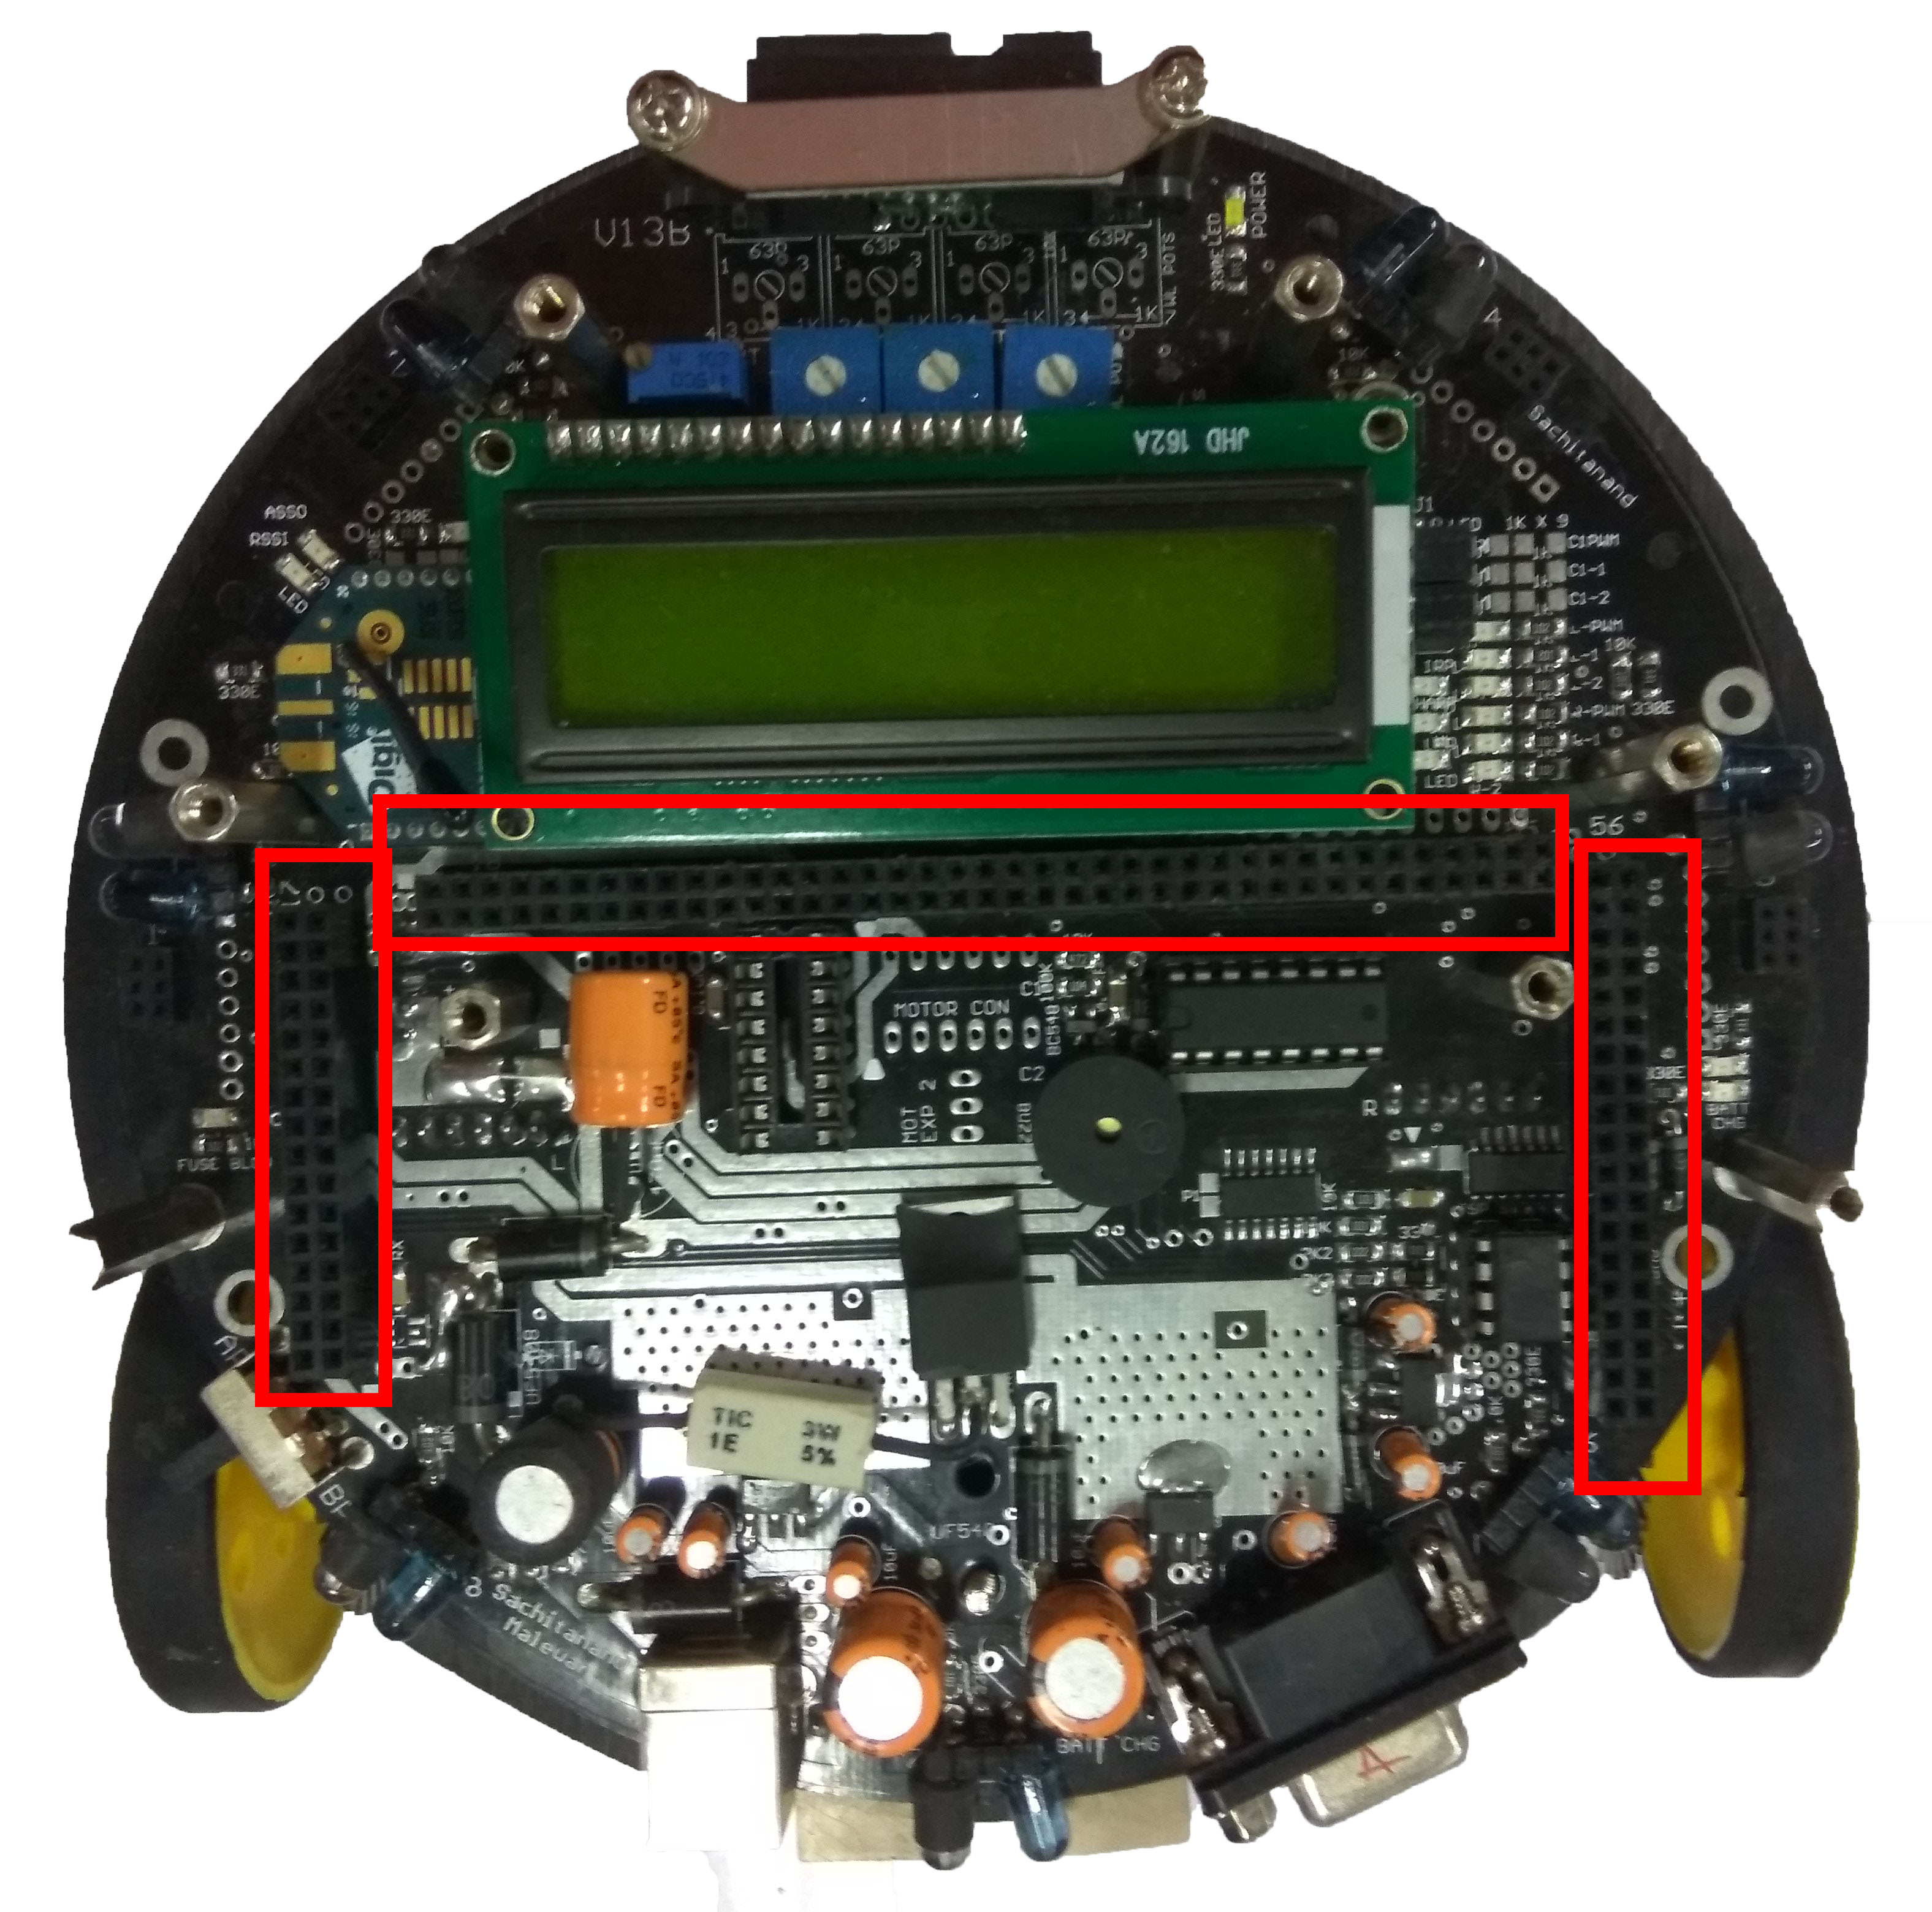
\includegraphics[width=6cm, height=6cm]{Images/3}
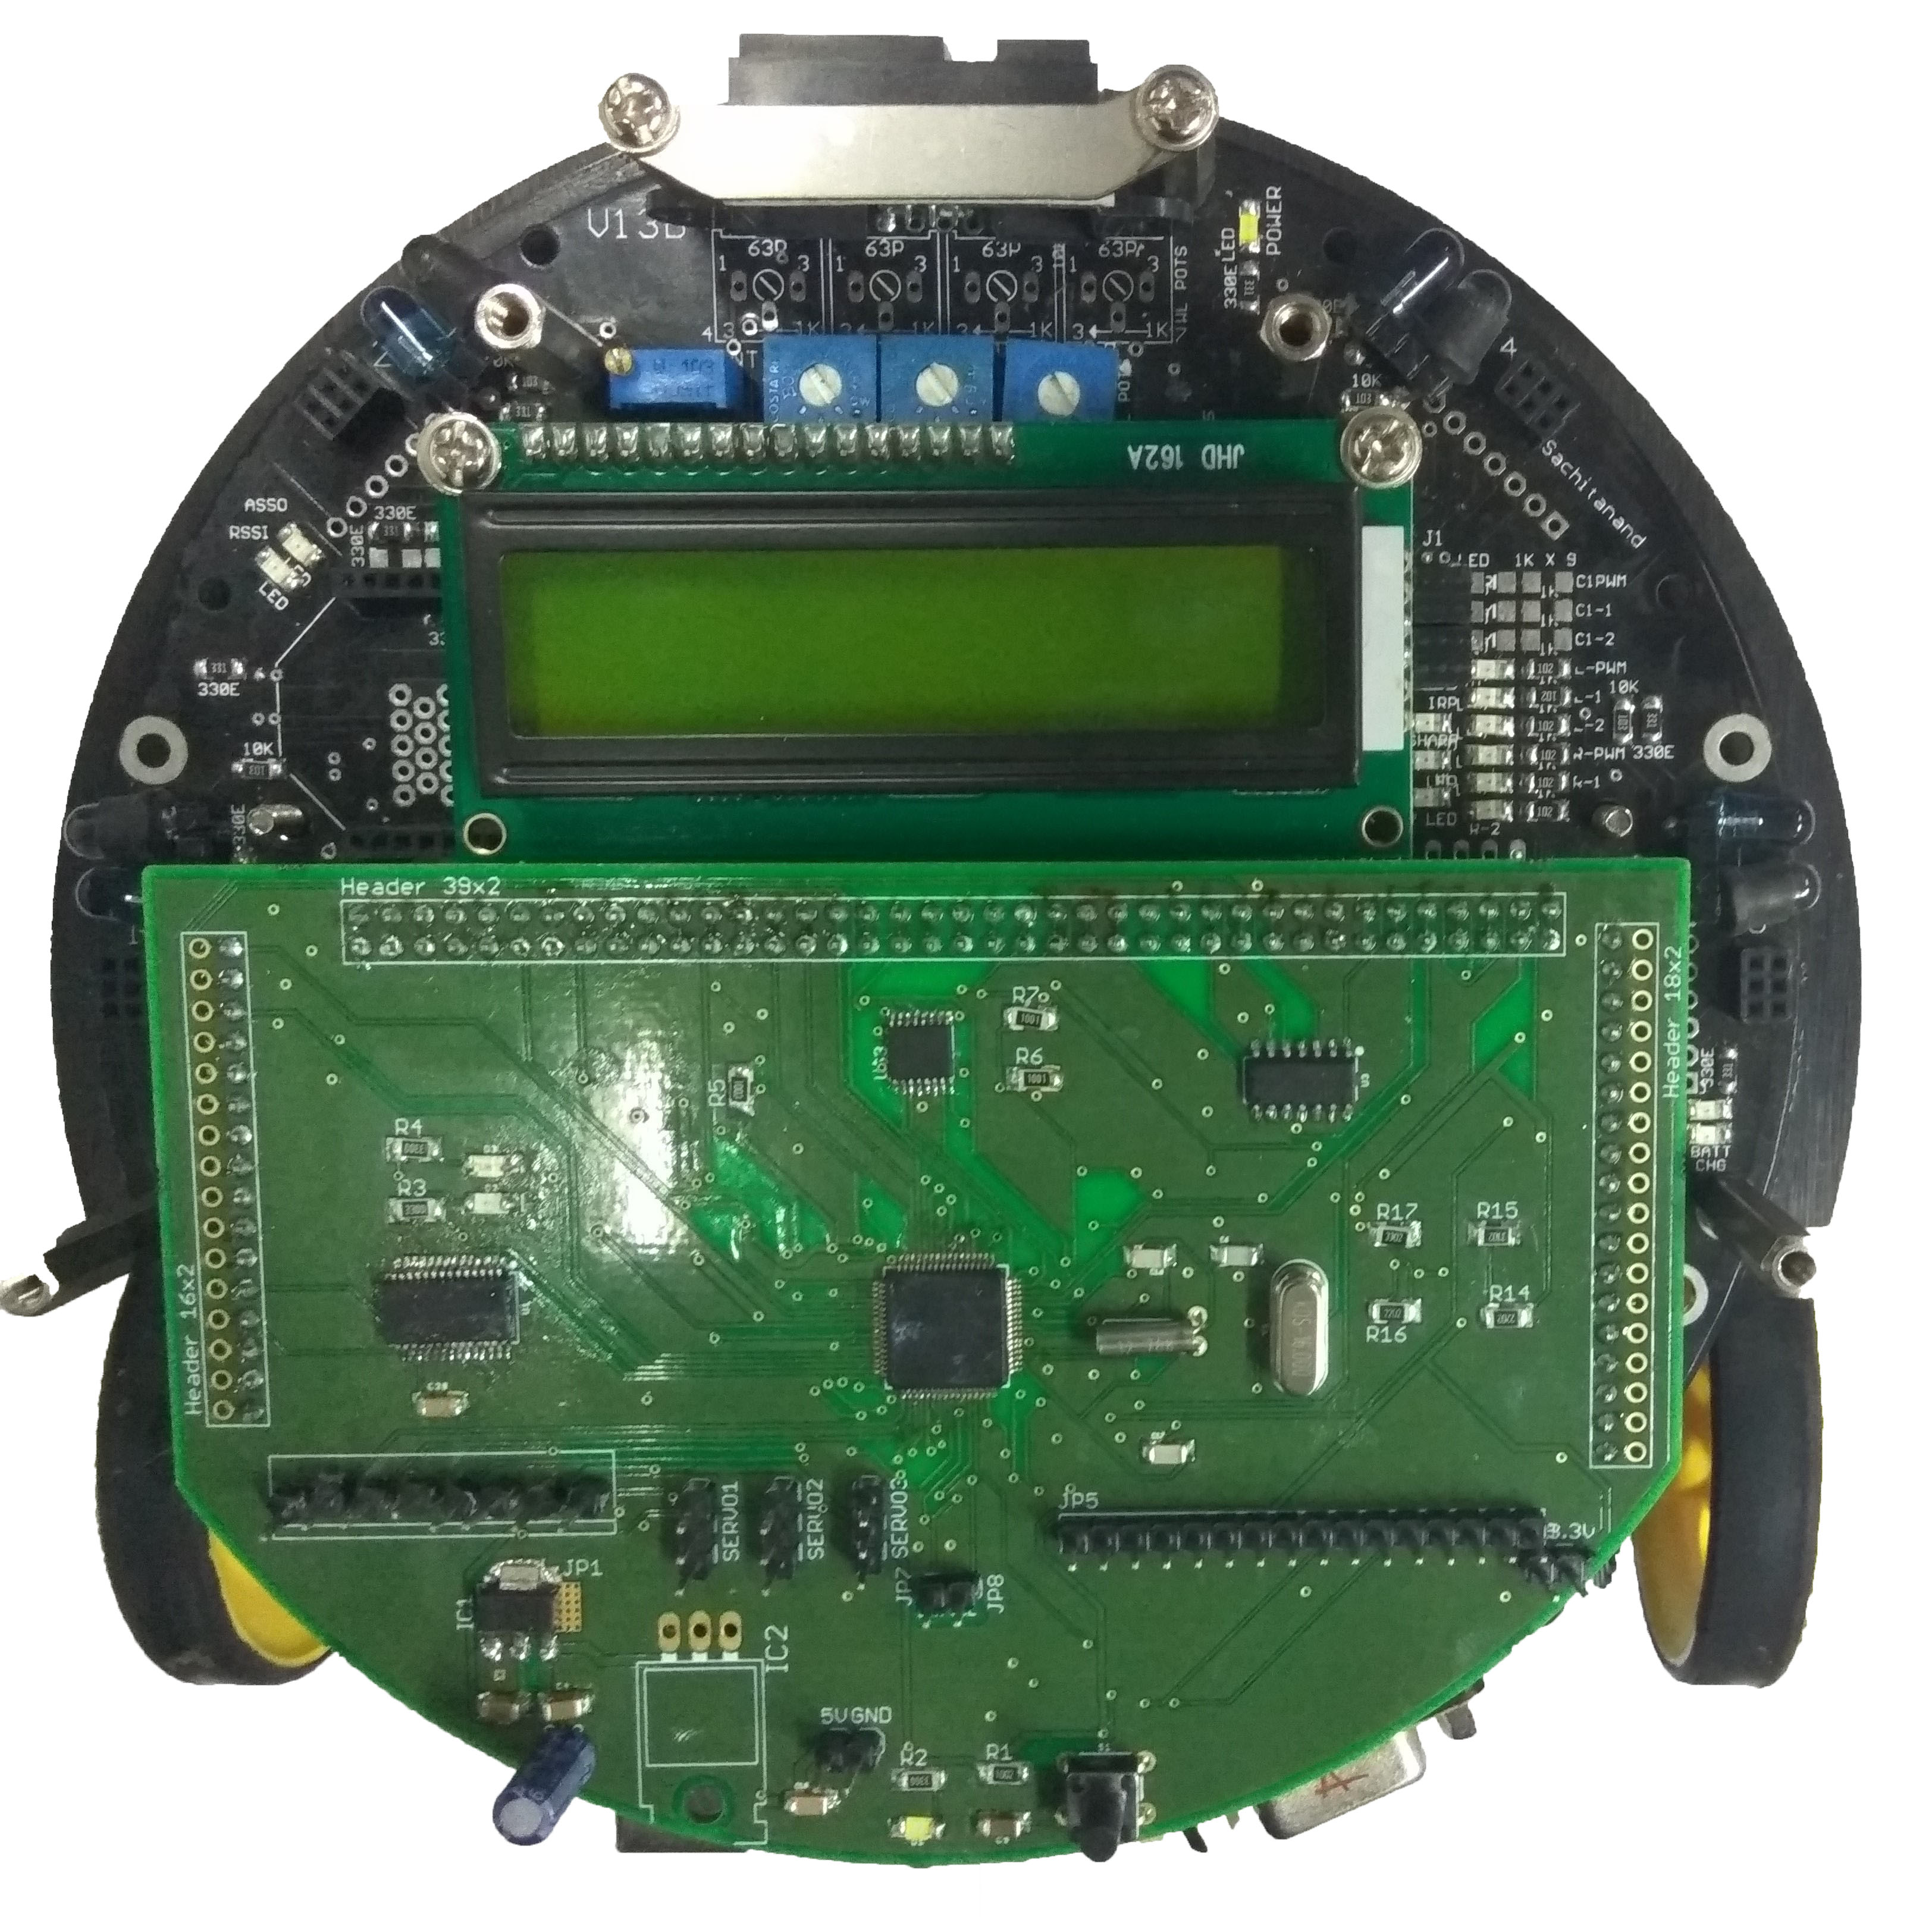
\includegraphics[width=6cm, height=6cm]{Images/4}\\

\hspace{2cm}
Figure24
\hspace{4.5cm}
Figure25

\section{Software and Code}
\href{http://www.github.com}{Github link} for the repository of code

%Brief explanation of various parts of code 


\section{Future Work}
\begin{enumerate}
	\item Create GUIs for user-friendly interface.
	\item TI-RTOS can be used in real-time multitasking applications. 
	\item Programming through bootloader.
	\item The TIVA based Firebird V can be extensively used for prototyping. 
	\item Real time debugger hence can be used in algorithm testing. 
\end{enumerate}

\section{Bug report and Challenges}
	\subsection{Bug report}
		\textbf{Plug and Play Board Version 1:}
		\begin{enumerate}
			\item 7805 Placement: The 7805 was not positioned at the end. Becuase of this there was no sufficient space to add the heat sink. 
			\item Port Expander Naming: The names of port expander are interchanged in the Daughter board. The names of port expander printed on the Daughter board are interchanged. Port B is named as port A and vice versa. 
			\item Switch Connection : The switch is used to connect the Ground of Launchpad and Daughter board for programming. The connections of this switch is incorrect.
			\item The bot has to powered first and then micro USB should be connected to program the bot. This is because of the absence of switch explained in the previous step 
			\item LCD starts displaying data on alternate press of reset button. It gets initialised everytime but fails to display data.
			\item Buzzer and red LED of TIVA launchad are on the same pin. Certain motors pins and red and green LED pins also overlap.
		\end{enumerate}
	All these errors are rectified in the version 2 of Plug and Play board. 
		\textbf{uC based board :}
		\begin{enumerate}
			\item RX and TX LEDs: LEDs attached to RX and TX pins of serial communication are not woring. The bot is able to communicate with the laptop serial but the LEDs are not glowing.
			\item Crystal Placement: The Crystal is placed far from the microcontroller. Because of this the inductance of wires may effect the crysal frequency. 
			\item Heat Sink: The heat sink provided for LM1117 is not sufficient. 
			\item Naming : The names of port expamders, servo headers, programming headers are not printer on the board. The names of SCL and SDA pins on the board is interchanged i.e SCL pin is printed as SDA and vice versa.
			\item The bot does not get programmed everytime because of connection problems.(Resolderig the pins of uC might help solve the problem)
			\item LCD starts displaying data on alternate press of reset button. It gets initialised everytime but fails to display data.
		\end{enumerate}
	\subsection{Challenges Faced}
		\begin{enumerate}
			\item Voltage Incompatibility: Firebird operates at 5v and TIVA board operates at 3.3v. So to interface TIVA board with Firebird V, we need level converters. The first one uses a diode in reverse bias condition to convert 5v to 3.3v. The second one uses BJT in cut off and active region to bring about the same functionality. By replacing BJT with MOSFET, it acts as a bidirectional level converter. Commercially this is available as BSS138.
			\item Unavailability of Firmware for programming TM4C123GH6: The TIVA Launchpad has two arm Cortex M4 microcontrollers. One of the controllers is specifically used for programming the general purpose controller. But the firmware for this is not open-source. So, it was decided that there will two different schematics of daughter board will be created.The first one will be a simple plug and play board using TIVA Launchpad as the main board. The other one will be a board that is completely designed on the single PCB with an external programming circuitry.
			\item Limited number of ADC Channels: Due to 12 ADC channels on TM4C123GH6PM controller, all the sensors on the firebird can not be interfaced directly. So an external ADC chip that works on I2C protocol will be interfaced with the daughter board to include all the sensors. After a thorough discussion, "ADC128D818 " was chosen. This has a 12-bit precision with 8 channels and can be interfaced using I2C communication, hence requires only 2 pins to be interfaced.
			\item Voltage Divider: The sharp sensors present on the Firebird operate on 5 volts i.e their output varies from 0-5v depending on the position of the obstacle. So there is a need for voltage divider, but the traditional voltage works on the assumption that there is no current drawn from the dividing node. Hence a buffer is used to stop the current. Again there are two choices, BJT in common collector mode and opamp. \\
			Simulating the above two circuit in Proteus, Common collector BJT has a gain of around 0.8 and opamp had a gain of around 1. Hence opamp is used in this board.
			\item Soldering the SMD components on the board.
		\end{enumerate}
\begin{thebibliography}{li}
	\item TIVA and code composer studio from the following sources 
	\begin{itemize}
		\item \href{https://www.google.co.in/url?sa=t\&rct=j\&q=\&esrc=s\&source=web\&cd=3\&sqi=2\&ved=0ahUKEwimtoeU5PHUAhWHpo8KHZmoCQ4QFgg1MAI\&url=https\%3A\%2F\%2Fwww.cse.iitb.ac.in\%2F~erts\%2Fhtml\_pages\%2FResources\%2FTiva\%2FTM4C123G_LaunchPad_Workshop_Workbook.pdf\&usg=AFQjCNGfuNP0-MWklzZhTATrZNd4aIE92Q\&cad=rja}{TM4C123G LaunchPad Workshop}
		\item \href{https://www.google.co.in/url?sa=t\&rct=j\&q=\&esrc=s\&source=web\&cd=4\&cad=rja\&uact=8\&sqi=2\&ved=0ahUKEwj3kvH15fHUAhXDtY8KHUVXAD8QFgg9MAM\&url=https\%3A\%2F\%2Fwww.cse.iitb.ac.in\%2F~erts\%2Fhtml\_pages\%2FResources\%2FTiva\%2FTM4C123G_LaunchPad_Workshop_Workbook.pdf\&usg=AFQjCNGfuNP0-MWklzZhTATrZNd4aIE92Q}{Workshop By IITB}
		\end{itemize}
	\item Eagle tutorial from this \href{https://www.youtube.com/watch?v=1AXwjZoyNno}{link} 
	
\end{thebibliography}


\end{document}

